\section{Introducción}

En este trabajo se presenta el desarrollo de un proyecto para una \textit{Huerta Orgánica de Precisión} (HOP) el cual incluyó una planificación utilizando metodologías ágiles ($Scrum$), un diseño orientado a objetos y una primera implementación en \verb|Python|. El objetivo del presente informe es detallar la experiencia del grupo utilizando la técnica de planificación en contraste con la puesta en práctica del desarrollo, así como también profundizar en algunas decisiones tomadas respecto del modelado y uso de ciertos patrones de diseño interesantes. Por último, se busca también documentar mínimamente la implementación y la batería de tests incluída para verificar los criterios de aceptación iniciales. 

\section{Planificación}

Para la planificación de este proyecto se utilizó la técnica $Scrum$ del ámbito de las metodologías ágiles. Para llevarla adelante se decidió utilizar la plataforma \textsl{RallyDev}, la cual sirvió como herramienta para cargar las \textit{User Stories} con sus respectivas tareas y criterios de aceptación, diagramar un primer \textit{Sprint} que traccionaría el desarrollo de este trabajo y llevar adelante un \textit{Burndown} de las tareas y las horas invertidas según lo planificado.\\
\indent Si bien la ténica no exige la utilización de esta herramienta, resultó de gran utilidad para poder poner el foco en lo que había que planificar, es decir identificar roles, stories, tareas, esfuerzo, etc., y no tanto en el soporte o las formalidades de la misma, algo ventajoso tratándose de la primera experiencia con la metodología.

\subsection{Product Backlog}

Como primera medida para la identificación de las $stories$ a desarrollar, y con la mira puesta en contextualizar el uso de la HOP, definimos los siguientes roles para la aplicación:

\begin{itemize}
\item \textbf{Botánico}: Es quien se encarga de diseñar el plan de cultivo, crecimiento y cuidado de las plantas, pudiendo realizar cambios sobre la marcha si fuera necesario.
\item \textbf{Jardinero}: Es quien se encarga de llevar a la práctica el plan diseñado por el botánico, realizar las tareas manuales de jardinería y llevar un monitoreo más técnico que el del consumidor.
\item \textbf{Consumidor}: es el que paga la semilla, los insumos y es dueño de los cultivos. Su interés es que todo salga bien para poder hacer usufructo de los mismos, por lo tanto debe monitorear los gastos, el estado de las plantas y saber cuándo podrá cosechar.
\end{itemize}

Es interesante notar que la distinción de roles no implica que, en la práctica, se trate de sujetos / usuarios distintos. Sin embargo, plantear el uso de la aplicación desde distintos puntos de vista resultó importante para poder visualizar las distintas funcionalidades que se desarrollarían, lo cual facilitó la decantación de las siguientes $user\ stories$ iniciales:

\begin{itemize}
\item Como Jardinero quiero ordenar a los actuadores que suministren insumos a la planta
\item Como Jardinero quiero visualizar el estado de los sensores
\item Como Jardinero quiero visualizar el plan de suministro de las siguientes 24hrs
\item Como Jardinero quiero visualizar el estado de la central meteorológica	
\item Como Botánico quiero modificar el programa de suministros 
\item Como Botánico quiero visualizar el estado de fenología	
\item Como Consumidor quiero visualizar el plan maestro	
\item Como Jardinero quiero ingresar estados de fenología	
\item Como Botánico quiero declarar un plan maestro de cultivo
\item Como Botánico quiero programar suministros de insumos
\end{itemize}

\subsection{Definición del Sprint}

Luego de la identificación de un conjunto de historias lo suficientemente robusto como para cubrir las funcionalidades y escenarios planteados en el documento que dio origen a este proyecto, se procedió a la elección de algunas de ellas para conformar el primer y único $sprint$ del desarrollo. El criterio de selección se realizó según lo indica la técnica empleada, asignando medidas de relación y esfuerzo a cada historia y luego tomando las primeras de un órden de mérito realizado según la relación entre ambas métricas. Este corte sí resultó más subjetivo, basado en las restricciones temporales y en la evaluación grupal que se hizo de las funcionalidades más importantes o pedidas dentro de las del ranking.

\begin{center}
    \begin{tabular}{ | c | p{5cm} | l | l |}
    \hline
    ID & Item & Business Value & Story Points \\ \hline
1 & Como Jardinero quiero ordenar a los actuadores que suministren insumos a la planta	& 7	& 1	\\ \hline
2 & Como Jardinero quiero visualizar el estado de los sensores	& 7 &	3 \\ \hline
3 & Como Jardinero quiero visualizar el plan de suministro de las siguientes 24hrs	& 7	& 3 \\ \hline
4 & Como Jardinero quiero visualizar el estado de la central meteorológica	& 6	& 3 \\ \hline
5 & Como Botánico quiero modificar el programa de suministros &	5	& 3 \\ \hline
6 & Como Botánico quiero visualizar el estado de fenología	& 4	& 3 \\ \hline
7 & Como Consumidor quiero visualizar el plan maestro	& 4	& 3 \\ \hline
8 & Como Jardinero quiero ingresar estados de fenología	& 6	& 5 \\ \hline
9 & Como Botánico quiero declarar un plan maestro de cultivo	& 7	& 8 \\ \hline
10 & Como Botánico quiero programar suministros de insumos	& 7	& 8 \\ \hline
    \end{tabular}
\end{center}

\subsection{Definición de Tareas}


\begin{description}
  \item[US79 Como Botánico quiero programar suministros de insumos] \hfill \\
  TA108	Desarrollo para ingreso de la programacion de suministro. horas estimadas $1$ \\
  TA109	Diseño Modulo que ejecuta suministros programados. horas estimadas $3$ \\
  TA208	Unit tests. horas estimadas $2$ \\
  TA209	Preparación Demo para la entrega. horas estimadas $2.5$
  \item[US75 Como Jardinero quiero visualizar el estado de los sensores] \hfill \\
	TA104	Desarrollo del diseño de los sensores. horas estimadas $1$ \\
	TA105	Implementación/Integración de la API con sensores (drivers, bibliotecas). horas estimadas $1$ \\
	TA106	Diseño del Modelo para almacenar y representar datos de los sensores (por ejemplo tempratura, humedad, etc). horas estimadas $1.5$ \\
	TA203	Unit tests. horas estimadas $1$ \\ 
  \item[US84 Como Botánico quiero declarar un plan maestro de cultivo] \hfill \\
  TA110	Diseño que soporte cambios en el plan maestro. horas estimadas $4$
  TA111	Permitir programación de estados de fenología y valores de indicadores esperados. horas estimadas $1$ \\
  TA128	Permitir programación de suministro de insumos. horas estimadas $2.5$ \\
  TA202	unit tests segun criterios de aceptación. horas estimadas $2$ \\
  TA205	Desarrollo de la implementación. horas estimadas $2$ \\
  \item[US78 Como Jardinero quiero visualizar el estado de la central meteorológica] \hfill \\
  TA112	Desarrollo del diseño de la central. horas estimadas $1$
  TA113	Implementación del modulo que se comunique con la API de la central meteorológica. horas estimadas $3.5$
  TA191	Modelo para la central. horas estimadas $1$
    \item[US90	Como Jardinero quiero ordenar a los actuadores que suministren insumos a la planta] \hfill \\\
    TA117	Modelo para la Integración entre API y actuadores (driver, biblioteca). horas estimadas $1$ \\
    TA125	Desarrollo del diseño que permita enviar mensajes a los actuadores. horas estimadas $1$ \\
    TA206	Implementación de la integracion. horas estimadas $2$ \\
  
    \item[US85 Como Botánico quiero visualizar el estadio de fenología] \hfill \\
    TA107	Desarrollo/Diseño para ver el estado de fenologia. horas estimadas $2$
    \item[US91	Como Jardinero quiero visualizar el plan de suministro de las siguientes 24hrs] \hfill \\
    	TA116	Funcionalidad para extraer del plan maestro datos de suministro de un próximo periodo. horas estimadas $3$
    
    \item[US87	Como Consumidor quiero visualizar el plan maestro] \hfill \\
    TA124	Desarrollo del modelo del plan maestro. horas estimadas $1.5$ \\
    TA190	Diseño/Modelo para el plan maestro. horas estimadas $1.5$ \\
    
        \item[US82	Como Jardinero quiero ingresar estados de fenología] \hfill \\
        TA126	Funcionalidad para definición de estados de fenología. horas estimadas $2$
        TA127	Permitir editar plan maestro para agregar estados de fenología definidos en la aplicación. horas estimadas $2$ \\
        TA207	Unit tests. horas estimadas $1$
        
         \item[US92	Como Botánico quiero modificar el programa de suministros] \hfill \\
         TA115	Desarrollo para soportar modificacion del programa. horas estimadas $2$
         
        

\end{description}

Inicialmente, este fue el análisis presentado para la estimación de trabajo en el sprint:\\

\indent \textsl{El equipo de trabajo se conforma por los 4 integrantes, quienes le dedicaríamos 2 horas por día de cursada a la realización del primer tramo del proyecto. Como en el sprint serán 8 días hábiles, en total cada uno aportaría 16 horas. Estimamos que un 15\% de ese tiempo reservado se pierde fuera del propósito de desarrollo principal, lo que nos da 13,60 horas reales por cada integrante durante esta etapa. En total se trata de 54,4 horas humanas entre todo el equpo.}\\
\indent \textsl{Por otro lado, las stories seleccionadas para el sprint suman 40 story points según la estimación de esfuerzo realizada. Como no contamos con un historial de otros sprints, definimos arbitrariamente que por cada story point se deberán consumir 1,2 horas de trabajo. Esto da 48 horas en total, dejando así 6,4 horas de margen en el caso de que la estimación no se cumpliera tal cual (probablemente) o hubiera que agregar otra story al sprint.}\\

\indent Vale aclarar que los 8 días hábiles pensados inicialmente no se concibieron de corrido, sino distribuidos a lo largo del tiempo asignado previo a la entrega final. De todas maneras se tuvieron que contemplar algunos días de fin de semana para utilizar algunas de las horas dejadas como margen para compensar algunos retrasos.

\subsection{Ejecución del Sprint}

A continuación mostraremos una burndown chart y un cumulative flow que muestran el desempeno del equipo a lo largo del primer sprint.

\begin{figure}[h!]
  \centering
  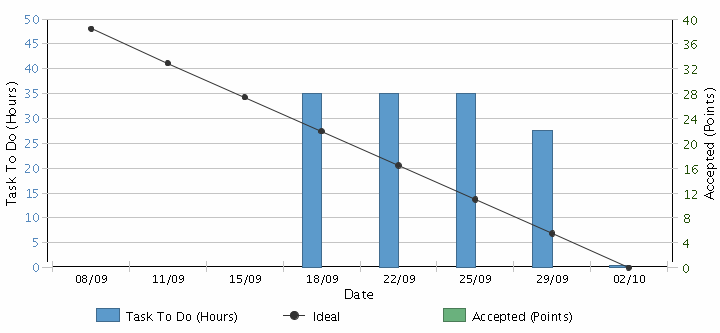
\includegraphics[width=0.8\textwidth]{./imagenes/burn_down.png}
  \caption{Burndown Chart}
  \label{fig:burn_down_chart}
\end{figure} 

A lo largo del desarrollo del sistema, el proyecto sufrió varios cambios. El principal eje de cambio fue el diseño general del sistema, esto se debió a la necedad de realizar un primer acercamiento grupal al dominio general del problema para poder entender de manera más detallada, el comportamiento y la funcionalidad del sistema que queríamos desarrollar. Esto generó algunos retrasos en el sprint que pudimos solucionar encontrando finalmente un diseño que nos resultó convincente. \\
En la segunda parte del sprint nos dedicamos al desarrollo de este diseño, por este motivo el grupo no alcanzo el rendimiento óptimo.

En el siguiente gráfico mostramos como fue la actividad del grupo a lo largo de la segunda parte del sprint.

\begin{figure}[h!]
  \centering
  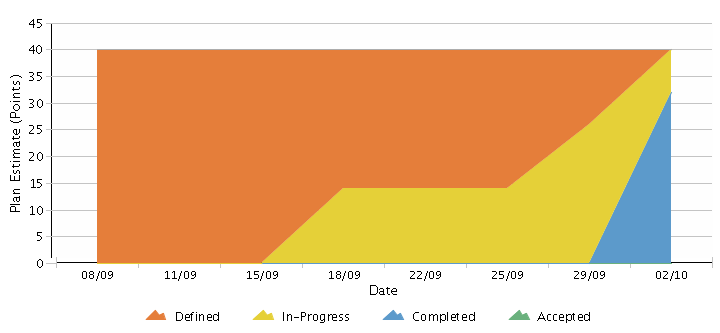
\includegraphics[width=0.8\textwidth]{./imagenes/cumulative_flow.png}
  \caption{Burndown Chart}
  \label{fig:cumulative_flow}
\end{figure} 



\subsection{Sprint Review}
Al ser inexpertos en el uso de la metodología, cometimos varios errores a lo largo del sprint, en particular relacionados con la distibución de tiempos por tarea. Como se observa en las imágenes de esta sección, pasamos varios días en discusiones previas sobre el diseño y reaizando poco avance a nivel de User Stories, y el avance que realizábamos no lo actualizábamos correspondientemente en la herramienta.
Con el correr de los días empezamos a marcar los avances realizados y a priorizar un poco más la completitud de algunas tareas, como se ve claramente en los

Habiendo cumplido el primer sprint finalizamos una primer versión del producto andando. 
La misma cuenta con las siguientes características:
\begin{itemize}
\item Recolección de datos de los sensores Arduino, la central meteorológica y el plan de suministro.
\item Elección de tareas a realizar en base a los datos recolectados.
\item Consulta al usuario para efectividad las acciones y automatización en caso de no existir una respuesta.
\item Actualización de los datos para verificar los cambios en el estado de la planta.
\end{itemize}

